\begin{figure}[!tb]
\centering
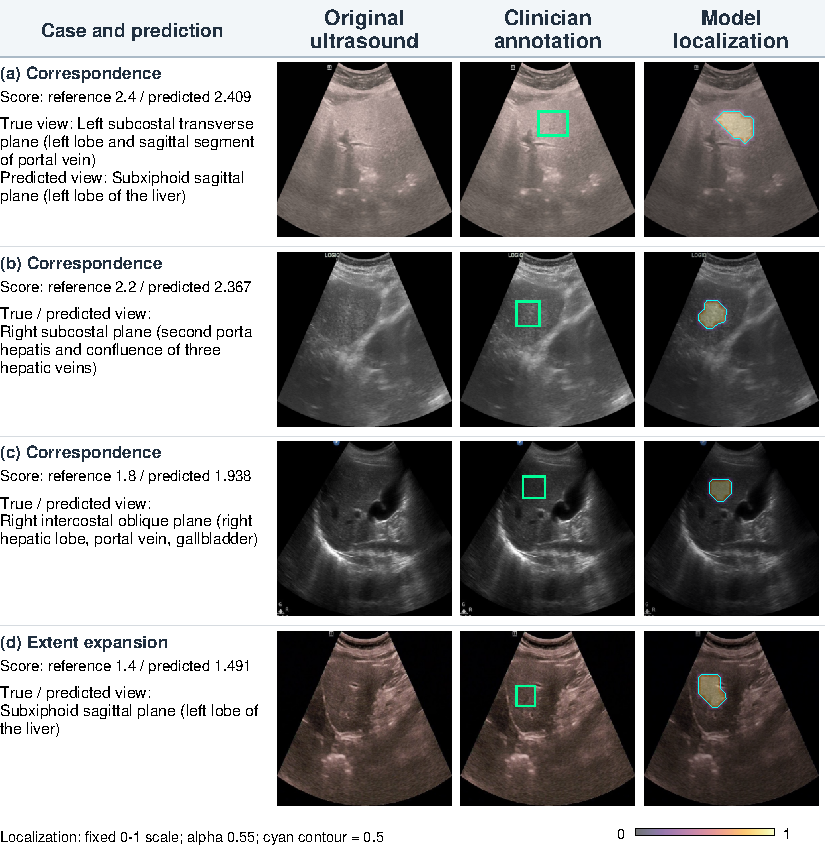
\includegraphics[width=\linewidth]{figures/assets/fig06_cases.pdf}
\caption{\lang{Four selected test cases, with reference and predicted scores and acquisition views at left. Predictions use the frozen checkpoint evaluated quantitatively. Rows (a)--(c) show localization correspondence; (d) shows a response beyond local boxes. Green boxes denote clinician annotations; localization uses a $[0,1]$ scale, opacity 0.55, and a cyan 0.5 contour. In row (a), the predicted view differs from the reference. These selected examples illustrate spatial outputs without establishing population localization performance or complete lesion extent.}{四个筛选的测试集病例，左侧标出参考及预测评分和扫查切面。预测使用参与定量评价的冻结检查点。(a)--(c) 展示定位对应，(d) 展示局部框外响应。绿色框为医生标注；定位色标为 $[0,1]$、透明度为 0.55，青色轮廓阈值为 0.5。(a) 的预测切面与参考切面不同。这些筛选示例用于展示空间输出，不代表总体定位水平或完整病灶范围。}}
\label{fig:cases}
\end{figure}
